\documentclass[12pt, a4paper]{article}

\usepackage[dvips]{graphics}
\usepackage{tabularx}
\usepackage{amsmath}
\usepackage{amsfonts}
\usepackage{amssymb}
\usepackage{graphicx}
\usepackage{float}
\usepackage{listings}
\usepackage{rotating}
\usepackage{tikz}
\usepackage{verbatim}
\pdfgentounicode=1

\begin{document}

\title{The FMB Algorithm}
\author{P. Baillehache}
\date{\today}
\maketitle

\begin{abstract}
This paper introduces how to perform intersection detection of pair of static/dynamic cuboid/tetrahedron in 2D/3D by using the Fourier-Motzkin elimination method.
\end{abstract}

\newpage
\tableofcontents

\section*{Introduction}

This paper introduces the FMB (Fourier-Motzkin-Baillehache) algorithm which can be used to perform intersection detection of moving and resting parallelepipeds and triangles in 2D, and cuboids and tetrahedrons in 3D.\\

The detection result is returned has a boolean (intersection / no intersection), and if there is intersection a bounding box of the intersection.\\

The two first sections introduce how the problem can be expressed as a system of linear inequation, and its resolution using the Fourier-Motzkin method.\\

The algorithm of the solution and its implementation in the C programming language are detailed in the four following sections.\\

The last two sections introduce the validation and qualification in term of relative performance of the FMB algorithm against the SAT algorithm.
 
\section{The problem as a system of linear inequations}

\subsection{Notations and definitions}

\begin{itemize}
\item{$\left[M\right]_{r,c}$ is the component at column $c$ and row $r$ of the matrix $M$}
\item{$\left[V\right]_r$ is the $r$-th component of the vector $\overrightarrow{V}$}
\item the term "frame" is used indifferently for parallelepiped, triangle, cuboid and tetrahedron.
\end{itemize}

\subsection{Static case}

The two Frames are represented as a vector origin and a number of component vectors equal to the dimension $D$ of the space where live the Frames. Each vector is of dimension equal to $D$.\\

Lets call $\mathbb{A}$ and $\mathbb{B}$ the two Frames tested for intersection. If $A$ and $B$ are two cuboids:
\begin{equation}
\mathbb{A}=\left\lbrace
\begin{array}{c}
\overrightarrow{X}\in[0.0,1.0]^D\\
\overrightarrow{O_\mathbb{A}}+C_\mathbb{A}.\overrightarrow{X}
\end{array}
\right\rbrace
\end{equation}
\begin{equation}
\mathbb{B}=\left\lbrace
\begin{array}{c}
\overrightarrow{X}\in[0.0,1.0]^D\\
\overrightarrow{O_\mathbb{B}}+C_\mathbb{B}.\overrightarrow{X}
\end{array}
\right\rbrace
\end{equation}
where $\overrightarrow{O_\mathbb{A}}$ is the origin of $\mathbb{A}$ and $C_\mathbb{A}$ is the matrix of the components of $A$ (one component per column). Idem for $\overrightarrow{O_\mathbb{B}}$ and $C_\mathbb{B}$.\\

If $\mathbb{A}$ and $\mathbb{B}$ are two tetrahedrons:
\begin{equation}
\mathbb{A}=\left\lbrace
\begin{array}{c}
\overrightarrow{X}\in[0.0,1.0]^D\\
\sum_{i=0}^{D-1}\left[X\right]_i\le1.0\\
\overrightarrow{O_\mathbb{A}}+C_\mathbb{A}.\overrightarrow{X}
\end{array}
\right\rbrace
\end{equation}
\begin{equation}
\mathbb{B}=\left\lbrace
\begin{array}{c}
\overrightarrow{X}\in[0.0,1.0]^D\\
\sum_{i=0}^{D-1}\left[X\right]_i\le1.0\\
\overrightarrow{O_\mathbb{B}}+C_\mathbb{B}.\overrightarrow{X}
\end{array}
\right\rbrace
\end{equation}

I'll assume the Frames are well formed, i.e. their components matrix is invertible. It is then possible to express $\mathbb{B}$ in $\mathbb{A}$'s coordinates system, noted as $\mathbb{B}_\mathbb{A}$. If $\mathbb{B}$ is a cuboid:
\begin{equation}
\mathbb{B}_\mathbb{A}=\left\lbrace
\begin{array}{c}
\overrightarrow{X}\in[0.0,1.0]^D\\
C_\mathbb{A}^{-1}.(\overrightarrow{O_\mathbb{B}}-\overrightarrow{O_\mathbb{A}}+C_\mathbb{B}.\overrightarrow{X})
\end{array}
\right\rbrace
\end{equation}

If $\mathbb{B}$ is a tetrahedron:
\begin{equation}
\mathbb{B}_\mathbb{A}=\left\lbrace
\begin{array}{c}
\overrightarrow{X}\in[0.0,1.0]^D\\
\sum_{i=0}^{D-1}\left[X\right]_i\le1.0\\
C_\mathbb{A}^{-1}.(\overrightarrow{O_\mathbb{B}}-\overrightarrow{O_\mathbb{A}}+C_\mathbb{B}.\overrightarrow{X})
\end{array}
\right\rbrace
\end{equation}

$\mathbb{A}$ in its own coordinates system becomes, for a cuboid:
\begin{equation}
\mathbb{A}_\mathbb{A}=\left\lbrace\overrightarrow{X}\in[0.0,1.0]^D\right\rbrace
\end{equation}
and for a tetrahedron:
\begin{equation}
\mathbb{A}_\mathbb{A}=\left\lbrace
\begin{array}{c}
\overrightarrow{X}\in[0.0,1.0]^D\\
\sum_{i=0}^{D-1}\left[X\right]_i\le1.0
\end{array}
\right\rbrace
\end{equation}

The intersection of $\mathbb{A}$ and $\mathbb{B}$ in $\mathbb{A}$'s coordinates sytem, can then be expressed as follow.\\

If $\mathbb{A}$ and $\mathbb{B}$ are two cuboids:
\begin{equation}
\left\lbrace
\begin{array}{c}
\overrightarrow{X}\in[0.0,1.0]^D\\
C_\mathbb{A}^{-1}.\left(\overrightarrow{O_\mathbb{B}}-\overrightarrow{O_\mathbb{A}}+C_\mathbb{B}.\overrightarrow{X}\right)\cap[0.0,1.0]^D
\end{array}
\right\rbrace
\end{equation}

If $\mathbb{A}$ is a cuboid and $\mathbb{B}$ is a tetrahedron:
\begin{equation}
\left\lbrace
\begin{array}{c}
\overrightarrow{X}\in[0.0,1.0]^D\\
\sum_{i=0}^{D-1}\left[X\right]_i\le1.0\\
C_\mathbb{A}^{-1}.\left(\overrightarrow{O_\mathbb{B}}-\overrightarrow{O_\mathbb{A}}+C_\mathbb{B}.\overrightarrow{X}\right)\cap[0.0,1.0]^D
\end{array}
\right\rbrace
\end{equation}

If $\mathbb{A}$ is a tetrahedron and $\mathbb{B}$ is a cuboid:
\begin{equation}
\left\lbrace
\begin{array}{c}
\overrightarrow{X}\in[0.0,1.0]^D\\
C_\mathbb{A}^{-1}.\left(\overrightarrow{O_\mathbb{B}}-\overrightarrow{O_\mathbb{A}}+C_\mathbb{B}.\overrightarrow{X}\right)\cap[0.0,1.0]^D\\
\sum_{i=0}^{D-1}\left[C_\mathbb{A}^{-1}.\left(\overrightarrow{O_\mathbb{B}}-\overrightarrow{O_\mathbb{A}}+C_\mathbb{B}.\overrightarrow{X}\right)\right]_i\le1.0\\
\end{array}
\right\rbrace
\end{equation}

If $\mathbb{A}$ and $\mathbb{B}$ are two tetrahedrons:
\begin{equation}
\left\lbrace
\begin{array}{c}
\overrightarrow{X}\in[0.0,1.0]^D\\
\sum_{i=0}^{D-1}\left[X\right]_i\le1.0\\
C_\mathbb{A}^{-1}.(\overrightarrow{O_\mathbb{B}}-\overrightarrow{O_\mathbb{A}}+C_\mathbb{B}.\overrightarrow{X})\cap[0.0,1.0]^D\\
\sum_{i=0}^{D-1}\left[C_\mathbb{A}^{-1}.\left(\overrightarrow{O_\mathbb{B}}-\overrightarrow{O_\mathbb{A}}+C_\mathbb{B}.\overrightarrow{X}\right)\right]_i\le1.0\\
\end{array}
\right\rbrace
\end{equation}

These can in turn be expressed as systems of linear inequations as follows, given the two shortcuts $\overrightarrow{O_{\mathbb{B}_\mathbb{A}}}=C_\mathbb{A}^{-1}.(\overrightarrow{O_\mathbb{B}}-\overrightarrow{O_\mathbb{A}})$ and $C_{\mathbb{B}_\mathbb{A}}=C_\mathbb{A}^{-1}.C_{\mathbb{B}}$.

If $\mathbb{A}$ and $\mathbb{B}$ are two cuboids:
\begin{equation}
\left\lbrace
\begin{array}{rcl}
\left[X\right]_0&\le&1.0\\
...\\
\left[X\right]_{D-1}&\le&1.0\\
-\left[X\right]_0&\le&0.0\\
...\\
-\left[X\right]_{D-1}&\le&0.0\\
\sum_{i=0}^{D-1}\left[C_{\mathbb{B}_\mathbb{A}}\right]_{0,i}.\left[X\right]_i&\le&1.0-\left[O_{\mathbb{B}_\mathbb{A}}\right]_0\\
...\\
\sum_{i=0}^{D-1}\left[C_{\mathbb{B}_\mathbb{A}}\right]_{D-1,i}.\left[X\right]_i&\le&1.0-\left[O_{\mathbb{B}_\mathbb{A}}\right]_{D-1}\\
-\sum_{i=0}^{D-1}\left[C_{\mathbb{B}_\mathbb{A}}\right]_{0,i}.\left[X\right]_i&\le&\left[O_{\mathbb{B}_\mathbb{A}}\right]_0\\
...\\
-\sum_{i=0}^{D-1}\left[C_{\mathbb{B}_\mathbb{A}}\right]_{D-1,i}.\left[X\right]_i&\le&\left[O_{\mathbb{B}_\mathbb{A}}\right]_{D-1}
\end{array}
\right.
\end{equation}

If $\mathbb{A}$ is a cuboid and $\mathbb{B}$ is a tetrahedron:
\begin{equation}
\left\lbrace
\begin{array}{rcl}
-\left[X\right]_0&\le&0.0\\
...\\
-\left[X\right]_{D-1}&\le&0.0\\
\sum_{i=0}^{D-1}\left[C_{\mathbb{B}_\mathbb{A}}\right]_{0,i}.\left[X\right]_i&\le&1.0-\left[O_{\mathbb{B}_\mathbb{A}}\right]_0\\
...\\
\sum_{i=0}^{D-1}\left[C_{\mathbb{B}_\mathbb{A}}\right]_{D-1,i}.\left[X\right]_i&\le&1.0-\left[O_{\mathbb{B}_\mathbb{A}}\right]_{D-1}\\
-\sum_{i=0}^{D-1}\left[C_{\mathbb{B}_\mathbb{A}}\right]_{0,i}.\left[X\right]_i&\le&\left[O_{\mathbb{B}_\mathbb{A}}\right]_0\\
...\\
-\sum_{i=0}^{D-1}\left[C_{\mathbb{B}_\mathbb{A}}\right]_{D-1,i}.\left[X\right]_i&\le&\left[O_{\mathbb{B}_\mathbb{A}}\right]_{D-1}\\
\sum_{i=0}^{D-1}\left[X\right]_i&\le&1.0
\end{array}
\right.
\end{equation}

If $\mathbb{A}$ is a tetrahedron and $\mathbb{B}$ is a cuboid:
\begin{equation}
\left\lbrace
\begin{array}{rcl}
\left[X\right]_0&\le&1.0\\
...\\
\left[X\right]_{D-1}&\le&1.0\\
-\left[X\right]_0&\le&0.0\\
...\\
-\left[X\right]_{D-1}&\le&0.0\\
-\sum_{i=0}^{D-1}\left[C_{\mathbb{B}_\mathbb{A}}\right]_{0,i}.\left[X\right]_i&\le&\left[O_{\mathbb{B}_\mathbb{A}}\right]_0\\
...\\
-\sum_{i=0}^{D-1}\left[C_{\mathbb{B}_\mathbb{A}}\right]_{D-1,i}.\left[X\right]_i&\le&\left[O_{\mathbb{B}_\mathbb{A}}\right]_{D-1}\\
\sum_{j=0}^{D-1}\left(\left(\sum_{i=0}^{D-1}\left[C_{\mathbb{B}_\mathbb{A}}\right]_{j,i}\right).\left[X\right]_i\right)&\le&1.0-\sum_{i=0}^{D-1}\left[O_{\mathbb{B}_\mathbb{A}}\right]_i
\end{array}
\right.
\end{equation}

If $\mathbb{A}$ and $\mathbb{B}$ are two tetrahedrons:
\begin{equation}
\left\lbrace
\begin{array}{rcl}
-\left[X\right]_0&\le&0.0\\
...\\
-\left[X\right]_{D-1}&\le&0.0\\
-\sum_{i=0}^{D-1}\left[C_{\mathbb{B}_\mathbb{A}}\right]_{0,i}.\left[X\right]_i&\le&\left[O_{\mathbb{B}_\mathbb{A}}\right]_0\\
...\\
-\sum_{i=0}^{D-1}\left[C_{\mathbb{B}_\mathbb{A}}\right]_{D-1,i}.\left[X\right]_i&\le&\left[O_{\mathbb{B}_\mathbb{A}}\right]_{D-1}\\
\sum_{i=0}^{D-1}\left[X\right]_i&\le&1.0\\
\sum_{j=0}^{D-1}\left(\left(\sum_{i=0}^{D-1}\left[C_{\mathbb{B}_\mathbb{A}}\right]_{j,i}\right).\left[X\right]_i\right)&\le&1.0-\sum_{i=0}^{D-1}\left[O_{\mathbb{B}_\mathbb{A}}\right]_i
\end{array}
\right.
\end{equation}

\subsection{Dynamic case}

If the frames $\mathbb{A}$ and $\mathbb{B}$ are moving linearly along the vectors $\overrightarrow{V_\mathbb{A}}$ and $\overrightarrow{V_\mathbb{B}}$ respectively during the interval of time $t\in[0.0,1.0]$, the above definition of the problem is modified as follow.\\

If $A$ and $B$ are two cuboids:
\begin{equation}
\mathbb{A}=\left\lbrace
\begin{array}{c}
\overrightarrow{X}\in[0.0,1.0]^D\\
t\in[0.0,1.0]\\
\overrightarrow{O_\mathbb{A}}+C_\mathbb{A}.\overrightarrow{X}+\overrightarrow{V_\mathbb{A}}.t
\end{array}
\right\rbrace
\end{equation}
\begin{equation}
\mathbb{B}=\left\lbrace
\begin{array}{c}
\overrightarrow{X}\in[0.0,1.0]^D\\
t\in[0.0,1.0]\\
\overrightarrow{O_\mathbb{B}}+C_\mathbb{B}.\overrightarrow{X}+\overrightarrow{V_\mathbb{B}}.t
\end{array}
\right\rbrace
\end{equation}
where $\overrightarrow{O_\mathbb{A}}$ is the origin of $\mathbb{A}$ and $C_\mathbb{A}$ is the matrix of the components of $A$ (one component per column). Idem for $\overrightarrow{O_\mathbb{B}}$ and $C_\mathbb{B}$.\\

If $\mathbb{A}$ and $\mathbb{B}$ are two tetrahedrons:
\begin{equation}
\mathbb{A}=\left\lbrace
\begin{array}{c}
\overrightarrow{X}\in[0.0,1.0]^D\\
t\in[0.0,1.0]\\
\sum_{i=0}^{D-1}\left[X\right]_i\le1.0\\
\overrightarrow{O_\mathbb{A}}+C_\mathbb{A}.\overrightarrow{X}+\overrightarrow{V_\mathbb{A}}.t
\end{array}
\right\rbrace
\end{equation}
\begin{equation}
\mathbb{B}=\left\lbrace
\begin{array}{c}
\overrightarrow{X}\in[0.0,1.0]^D\\
t\in[0.0,1.0]\\
\sum_{i=0}^{D-1}\left[X\right]_i\le1.0\\
\overrightarrow{O_\mathbb{B}}+C_\mathbb{B}.\overrightarrow{X}+\overrightarrow{V_\mathbb{B}}.t
\end{array}
\right\rbrace
\end{equation}

If $\mathbb{B}$ is a cuboid, $\mathbb{B}_\mathbb{A}$ becomes:
\begin{equation}
\mathbb{B}_\mathbb{A}=\left\lbrace
\begin{array}{c}
\overrightarrow{X}\in[0.0,1.0]^D\\
t\in[0.0,1.0]\\
C_\mathbb{A}^{-1}.\left(\overrightarrow{O_\mathbb{B}}-\overrightarrow{O_\mathbb{A}}+C_\mathbb{B}.\overrightarrow{X}+\left(\overrightarrow{V_\mathbb{B}}-\overrightarrow{V_\mathbb{A}}\right).t\right)
\end{array}
\right\rbrace
\end{equation}

If $\mathbb{B}$ is a tetrahedron:
\begin{equation}
\mathbb{B}_\mathbb{A}=\left\lbrace
\begin{array}{c}
\overrightarrow{X}\in[0.0,1.0]^D\\
t\in[0.0,1.0]\\
\sum_{i=0}^{D-1}\left[X\right]_i\le1.0\\
C_\mathbb{A}^{-1}.\left(\overrightarrow{O_\mathbb{B}}-\overrightarrow{O_\mathbb{A}}+C_\mathbb{B}.\overrightarrow{X}+\left(\overrightarrow{V_\mathbb{B}}-\overrightarrow{V_\mathbb{A}}\right).t\right)
\end{array}
\right\rbrace
\end{equation}

$\mathbb{A}$ in its own coordinates system has the same definition as in the static case. For a cuboid:
\begin{equation}
\mathbb{A}_\mathbb{A}=\left\lbrace\overrightarrow{X}\in[0.0,1.0]^D\right\rbrace
\end{equation}
and for a tetrahedron:
\begin{equation}
\mathbb{A}_\mathbb{A}=\left\lbrace
\begin{array}{c}
\overrightarrow{X}\in[0.0,1.0]^D\\
\sum_{i=0}^{D-1}\left[X\right]_i\le1.0\end{array}
\right\rbrace
\end{equation}

The intersection of $\mathbb{A}$ and $\mathbb{B}$ in $\mathbb{A}$'s coordinates sytem, can then be expressed as follow.\\

If $\mathbb{A}$ and $\mathbb{B}$ are two cuboids:
\begin{equation}
\left\lbrace
\begin{array}{c}
\overrightarrow{X}\in[0.0,1.0]^D\\
t\in[0.0,1.0]\\
C_\mathbb{A}^{-1}.\left(\overrightarrow{O_\mathbb{B}}-\overrightarrow{O_\mathbb{A}}+C_\mathbb{B}.\overrightarrow{X}+\left(\overrightarrow{V_\mathbb{B}}-\overrightarrow{V_\mathbb{A}}\right).t\right)\cap[0.0,1.0]^D
\end{array}
\right\rbrace
\end{equation}

If $\mathbb{A}$ is a cuboid and $\mathbb{B}$ is a tetrahedron:
\begin{equation}
\left\lbrace
\begin{array}{c}
\overrightarrow{X}\in[0.0,1.0]^D\\
t\in[0.0,1.0]\\
\sum_{i=0}^{D-1}\left[X\right]_i\le1.0\\
C_\mathbb{A}^{-1}.\left(\overrightarrow{O_\mathbb{B}}-\overrightarrow{O_\mathbb{A}}+C_\mathbb{B}.\overrightarrow{X}+\left(\overrightarrow{V_\mathbb{B}}-\overrightarrow{V_\mathbb{A}}\right).t\right)\cap[0.0,1.0]^D
\end{array}
\right\rbrace
\end{equation}

If $\mathbb{A}$ is a tetrahedron and $\mathbb{B}$ is a cuboid:
\begin{equation}
\left\lbrace
\begin{array}{c}
\overrightarrow{X}\in[0.0,1.0]^D\\
t\in[0.0,1.0]\\
C_\mathbb{A}^{-1}.\left(\overrightarrow{O_\mathbb{B}}-\overrightarrow{O_\mathbb{A}}+C_\mathbb{B}.\overrightarrow{X}+\left(\overrightarrow{V_\mathbb{B}}-\overrightarrow{V_\mathbb{A}}\right).t\right)\cap[0.0,1.0]^D\\
\sum_{i=0}^{D-1}\left[C_\mathbb{A}^{-1}.\left(\overrightarrow{O_\mathbb{B}}-\overrightarrow{O_\mathbb{A}}+C_\mathbb{B}.\overrightarrow{X}\right)\right]_i\le1.0\\
\end{array}
\right\rbrace
\end{equation}

If $\mathbb{A}$ and $\mathbb{B}$ are two tetrahedrons:
\begin{equation}
\left\lbrace
\begin{array}{c}
\overrightarrow{X}\in[0.0,1.0]^D\\
t\in[0.0,1.0]\\
\sum_{i=0}^{D-1}\left[X\right]_i\le1.0\\
C_\mathbb{A}^{-1}.\left(\overrightarrow{O_\mathbb{B}}-\overrightarrow{O_\mathbb{A}}+C_\mathbb{B}.\overrightarrow{X}+\left(\overrightarrow{V_\mathbb{B}}-\overrightarrow{V_\mathbb{A}}\right).t\right)\cap[0.0,1.0]^D\\
\sum_{i=0}^{D-1}\left[C_\mathbb{A}^{-1}.\left(\overrightarrow{O_\mathbb{B}}-\overrightarrow{O_\mathbb{A}}+C_\mathbb{B}.\overrightarrow{X}\right)\right]_i\le1.0\\
\end{array}
\right\rbrace
\end{equation}

These lead to the following systems of linear inequations, given the three shortcuts $\overrightarrow{O_{\mathbb{B}_\mathbb{A}}}=C_\mathbb{A}^{-1}.(\overrightarrow{O_\mathbb{B}}-\overrightarrow{O_\mathbb{A}})$, $\overrightarrow{V_{\mathbb{B}_\mathbb{A}}}=C_\mathbb{A}^{-1}.(\overrightarrow{V_\mathbb{B}}-\overrightarrow{V_\mathbb{A}})$ and $C_{\mathbb{B}_\mathbb{A}}=C_\mathbb{A}^{-1}.C_{\mathbb{B}}$.

If $\mathbb{A}$ and $\mathbb{B}$ are two cuboids:
\begin{equation}
\left\lbrace
\begin{array}{rcl}
t&\le&1.0\\
-t&\le&0.0\\
\left[X\right]_0&\le&1.0\\
...\\
\left[X\right]_{D-1}&\le&1.0\\
-\left[X\right]_0&\le&0.0\\
...\\
-\left[X\right]_{D-1}&\le&0.0\\
\left[V_{\mathbb{B}_\mathbb{A}}\right]_0.t+\sum_{i=0}^{D-1}\left[C_{\mathbb{B}_\mathbb{A}}\right]_{0,i}\left[X\right]_i&\le&1.0-\left[O_{\mathbb{B}_\mathbb{A}}\right]_0\\
...\\
\left[V_{\mathbb{B}_\mathbb{A}}\right]_{D-1}.t+\sum_{i=0}^{D-1}\left[C_{\mathbb{B}_\mathbb{A}}\right]_{D-1,i}\left[X\right]_i&\le&1.0-\left[O_{\mathbb{B}_\mathbb{A}}\right]_{D-1}\\
-\left[V_{\mathbb{B}_\mathbb{A}}\right]_0.t-\sum_{i=0}^{D-1}\left[C_{\mathbb{B}_\mathbb{A}}\right]_{0,i}\left[X\right]_i&\le&\left[O_{\mathbb{B}_\mathbb{A}}\right]_0\\
...\\
-\left[V_{\mathbb{B}_\mathbb{A}}\right]_{D-1}.t-\sum_{i=0}^{D-1}\left[C_{\mathbb{B}_\mathbb{A}}\right]_{D-1,i}\left[X\right]_i&\le&\left[O_{\mathbb{B}_\mathbb{A}}\right]_{D-1}
\end{array}
\right.
\end{equation}

If $\mathbb{A}$ is a cuboid and $\mathbb{B}$ is a tetrahedron:
\begin{equation}
\left\lbrace
\begin{array}{rcl}
t&\le&1.0\\
-t&\le&0.0\\
-\left[X\right]_0&\le&0.0\\
...\\
-\left[X\right]_{D-1}&\le&0.0\\
\left[V_{\mathbb{B}_\mathbb{A}}\right]_0.t+\sum_{i=0}^{D-1}\left[C_{\mathbb{B}_\mathbb{A}}\right]_{0,i}\left[X\right]_i&\le&1.0-\left[O_{\mathbb{B}_\mathbb{A}}\right]_0\\
...\\
\left[V_{\mathbb{B}_\mathbb{A}}\right]_{D-1}.t+\sum_{i=0}^{D-1}\left[C_{\mathbb{B}_\mathbb{A}}\right]_{D-1,i}\left[X\right]_i&\le&1.0-\left[O_{\mathbb{B}_\mathbb{A}}\right]_{D-1}\\
-\left[V_{\mathbb{B}_\mathbb{A}}\right]_0.t-\sum_{i=0}^{D-1}\left[C_{\mathbb{B}_\mathbb{A}}\right]_{0,i}\left[X\right]_i&\le&\left[O_{\mathbb{B}_\mathbb{A}}\right]_0\\
...\\
-\left[V_{\mathbb{B}_\mathbb{A}}\right]_{D-1}.t-\sum_{i=0}^{D-1}\left[C_{\mathbb{B}_\mathbb{A}}\right]_{D-1,i}\left[X\right]_i&\le&\left[O_{\mathbb{B}_\mathbb{A}}\right]_{D-1}\\
\sum_{i=0}^{D-1}\left[X\right]_i&\le&1.0
\end{array}
\right.
\end{equation}

If $\mathbb{A}$ is a tetrahedron and $\mathbb{B}$ is a cuboid:
\begin{equation}
\left\lbrace
\begin{array}{rcl}
t&\le&1.0\\
-t&\le&0.0\\
\left[X\right]_0&\le&1.0\\
...\\
\left[X\right]_{D-1}&\le&1.0\\
-\left[X\right]_0&\le&0.0\\
...\\
-\left[X\right]_{D-1}&\le&0.0\\
-\sum_{i=0}^{D-1}\left[C_{\mathbb{B}_\mathbb{A}}\right]_{0,i}\left[X\right]_i&\le&\left[O_{\mathbb{B}_\mathbb{A}}\right]_0\\
...\\
-\left[V_{\mathbb{B}_\mathbb{A}}\right]_{D-1}.t-\sum_{i=0}^{D-1}\left[C_{\mathbb{B}_\mathbb{A}}\right]_{D-1,i}\left[X\right]_i&\le&\left[O_{\mathbb{B}_\mathbb{A}}\right]_{D-1}\\
\sum_{j=0}^{D-1}\left(\left[V_{\mathbb{B}_\mathbb{A}}\right]_j.t+\sum_{i=0}^{D-1}\left[C_{\mathbb{B}_\mathbb{A}}\right]_{j,i}\left[X\right]_i\right)&\le&1.0-\sum_{i=0}^{D-1}\left[O_{\mathbb{B}_\mathbb{A}}\right]_{i}
\end{array}
\right.
\end{equation}

If $\mathbb{A}$ and $\mathbb{B}$ are two tetrahedrons:
\begin{equation}
\left\lbrace
\begin{array}{rcl}
t&\le&1.0\\
-t&\le&0.0\\
-\left[X\right]_0&\le&0.0\\
...\\
-\left[X\right]_{D-1}&\le&0.0\\
-\sum_{i=0}^{D-1}\left[C_{\mathbb{B}_\mathbb{A}}\right]_{0,i}\left[X\right]_i&\le&\left[O_{\mathbb{B}_\mathbb{A}}\right]_{0}\\
...\\
-\left[V_{\mathbb{B}_\mathbb{A}}\right]_{D-1}.t-\sum_{i=0}^{D-1}\left[C_{\mathbb{B}_\mathbb{A}}\right]_{D-1,i}\left[X\right]_i&\le&\left[O_{\mathbb{B}_\mathbb{A}}\right]_{D-1}\\
\sum_{i=0}^{D-1}\left[X\right]_i&\le&1.0\\
\sum_{j=0}^{D-1}\left(\left[V_{\mathbb{B}_\mathbb{A}}\right]_j.t+\sum_{i=0}^{D-1}\left[C_{\mathbb{B}_\mathbb{A}}\right]_{j,i}\left[X\right]_i\right)&\le&1.0-\sum_{i=0}^{D-1}\left[O_{\mathbb{B}_\mathbb{A}}\right]_{i}
\end{array}
\right.
\end{equation}

\section{Resolution of the problem by Fourier-Motzkin method}

\subsection{The Fourier-Motzkin elimination method}

The Fourier-Motzkin elimination method has been introduced by J.J.-B. Fourier in 1827 \cite{fourier}, and described in the Ph.D. thesis of T.S. Motzkin in 1936 \cite{motzkin}. This is a generalization of the Gaussian elimination method to linear systems of inequalities. This method consists of eliminating one variable of the system and rewrite a new system accordingly. Then the elimination operation is repeated on another variable in the new system, and so on until we obtain a trivial system with only one variable. From there, a solution for each variable can be obtained if it exists. The variable elimination is performed as follow.\\
Lets write the linear system $\mathcal{I}$ of $m$ inequalities and $n$ variables as 
\begin{equation}
\left\{\
\begin{array}{ccccc}
a_{11}.x_1&+a_{12}.x_2&+\cdots&+a_{1n}.x_n &\le b_1\\
a_{21}.x_1&+a_{22}.x_2&+\cdots&+a_{2n}.x_n &\le b_2\\
&&\vdots&&\\
a_{m1}.x_1&+a_{m2}.x_2&+\cdots&+a_{mn}.x_n &\le b_m\\
\end{array}
\right.
\end{equation}
with
\begin{equation}
\begin{array}{c}
i\in{1, 2, ..., m}\\
j\in{1, 2, ..., n}\\
x_i\in\mathbb{R}\\
a_{ij}\in\mathbb{R}\\
b_j\in\mathbb{R} 
\end{array}
\end{equation}
To eliminate the first variable $x_1$, lets multiply each inequality by $1.0/|a_{i1}|$ where $a_{i1}\not=0.0$. The system becomes
\begin{equation}
\label{eqn_elim_system}
\left\{\
\begin{array}{ccccc}
x_1&+a'_{i2}.x_2&+\cdots&+a'_{in}.x_n &\le b'_i\qquad(i\in\mathcal{I}_+)\\
&a_{i2}.x_2&+\cdots&+a_{in}.x_n &\le b_i\qquad(i\in\mathcal{I}_0)\\
-x_1&+a'_{i2}.x_2&+\cdots&+a'_{in}.x_n &\le b'_i\qquad(i\in\mathcal{I}_-)\\
\end{array}
\right.
\end{equation}
where 
$$\mathcal{I}_+=\{i:a_{i1}>0.0\}$$
$$\mathcal{I}_0=\{i:a_{i1}=0.0\}$$
$$\mathcal{I}_-=\{i:a_{i1}<0.0\}$$
$$a'_{ij}=a_{ij}/|a_{i1}|$$
$$b'_i=b_i/|a_{i1}|$$
Then $x_1, x_2, \cdots, x_n\in\mathbb{R}^n$ is a solution of $\mathcal{I}$ if and only if
\begin{equation}
\left\{\
\begin{array}{c}
\sum_{j=2}^n((a'_{kj}+a'_{lj}).x_j)\le b'_k+b'_l \qquad (k\in\mathcal{I}_+, l\in\mathcal{I}_-)\\
\sum_{j=2}^n(a_{ij}.x_j)\le b_i \qquad i\in\mathcal{I}_0
\end{array}
\right.
\end{equation}
and
\begin{equation}
\max_{l\in\mathcal{I}_-}(\sum_{j=2}^n(a'_{lj}.x_j)-b'_l)\le x_1\le\min_{k\in\mathcal{I}_+}(b'_k-\sum_{j=2}^n(a'_{kj}.x_j))
\end{equation}
The same method is then applied on this new system to eliminate the second variable $x_2$, and so on until we reach the inequality
\begin{equation}
\max_{l\in\mathcal{I}^{''...'}_-}(-b^{''...'}_l)\le x_n\le\min_{k\in\mathcal{I}^{''...'}_+}(b^{''...'}_k)
\end{equation}
If this inequality has no solution, then neither the system $\mathcal{I}$. If it has a solution, the minimum and maximum are the bounding values for the variable $x_n$. One can get a particular solution to the system $\mathcal{I}$ by choosing a value for $x_n$ between these bounding values, which allow us to set a particular value for the variable $x_{n-1}$, and so on back up to $x_1$. 

\subsection{Application of the Fourier-Motzkin method to the intersection problem}

The Fourier-Motzkin method can be directly applied to obtain the bounds of each variable, if the system has a solution. If the system has no solution, the method will eventually reach an inconsistent inequality.\\

One solution $\overrightarrow{S}$ within the bounds obtained by the resolution of the system is expressed in the Frame $\mathbb{B}$'s coordinates system. One can get the equivalent coordinates $\overrightarrow{S'}$ in the real world's coordinates system as follow:
\begin{equation}
\overrightarrow{S'}=\overrightarrow{O_\mathbb{B}}+C_\mathbb{B}.\overrightarrow{S}
\end{equation}

Only one inconsistent inequality is sufficient to prove the absence of solution, and then the non intersection of the Frames. One shall check the inconsistence of each inequality as soon as possible during the resolution of the system to optimize the speed of the algorithm.\\

A suficient condition for one inequality $\sum_ia_iX_i\le Y$ to be inconsistent is, given that $\forall i,X_i\in[0.0,1.0]$:
\begin{equation}
Y<\sum_{i\in I^-}a_i
\end{equation}
where $I^-=\left\lbrace i, a_i<0.0\right\rbrace$.\\

\subsection{About the size of system of linear inequation}

During implementation in languages where the developper needs to manage memory itself the size of the systems (\ref{eqn_elim_system}) resulting from variable elimination is necessary but cannot be forecasted. Instead, a maximum size can be calculated as follow.\\

Lets call $n_-$, $n_+$ and $n_0$ the size of, respectively, $\mathcal{I}_-$, $\mathcal{I}_+$ and $\mathcal{I}_0$, and $N$ the number of inequalities in the original system and $N'$ the number inequalities in the resulting system. We have:\\
\begin{equation}
n_-+n_++n_0=N
\end{equation}
and
\begin{equation}
\label{eqn_def_N_prime}
n_-.n_++n_0=N'
\end{equation}
Now lets define $K=N-n_0$, then we have:\\
\begin{equation}
n_-+n_+=K
\end{equation}
then,
\begin{equation}
n_-.n_+=n_-(K-n_-)
\end{equation}
then,
\begin{equation}
n_-.n_+=K.n_-n_-^2
\end{equation}
The right part is polynomial whose maximum is reached for $n_-=K/2$. Then,
\begin{equation}
n_-.n_+\le K^2/2-K^2/4
\end{equation}
or,
\begin{equation}
n_-.n_+\le K^2/4
\end{equation}
and putting back the definition of $K$
\begin{equation}
n_-.n_+\le (N-n_0)^2/4
\end{equation}
which is also
\begin{equation}
n_-.n_+\le N^2/4
\end{equation}
From (\ref{eqn_def_N_prime}) we get,
\begin{equation}
N'\le N^2/4-n_0
\end{equation}
and getting rid of the $n_0$ knowing that $n_0\ge0$,
\begin{equation}
N'\le N^2/4
\end{equation}
The maximum number of inequation in the initial system is defined for each case (2D/3D, static/dynamic) in the previous section. This leads to the following maximum number of inequations:\\
$$
\begin{array}{|c|c|c|c|c|}
\hline
&N&N'&N''&N'''\\
\hline
2Dstatic&8&16&&\\
\hline
2Ddynamic&10&25&157&\\
\hline
3Dstatic&12&36&324&\\
\hline
3Ddynamic&14&49&601&90301\\
\hline
\end{array}
$$

\section{Algorithms of the solution}

In this section I introduce the algorithms of the solution of the previous section for each case (static/dynamic and 2D/3D), and the algorithms to manipulate the structure used to represent the cuboid and tetrahedron.\\

Algorithms are given in pseudo code, and consequently without any optimization based on properties of one given language. One can refer to the C implementation in the following sections for possible optimization in this language.\\

Algorithms are also given independantly from each other. Code commonalization may be possible if one plans to gather several cases together, but this is dependant of the implementation and thus left to the developper responsibility.\\

\subsection{2D static}

\begin{scriptsize}
\begin{ttfamily}
\lstinputlisting[breaklines]{../2D/algorithm.txt}
\end{ttfamily}
\end{scriptsize}

\subsection{3D static}

\begin{scriptsize}
\begin{ttfamily}
\lstinputlisting[breaklines]{../3D/algorithm.txt}
\end{ttfamily}
\end{scriptsize}

\subsection{2D dynamic}

\begin{scriptsize}
\begin{ttfamily}
\lstinputlisting[breaklines]{../2DTime/algorithm.txt}
\end{ttfamily}
\end{scriptsize}

\subsection{3D dynamic}

\begin{scriptsize}
\begin{ttfamily}
\lstinputlisting[breaklines]{../3DTime/algorithm.txt}
\end{ttfamily}
\end{scriptsize}

\section{Implementation of the algorithms in C}

In this section I introduce an implementation of the algorithms of the previous section in the C language.\\

\subsection{Frames}

\subsubsection{Header}

\begin{scriptsize}
\begin{ttfamily}
\lstinputlisting[breaklines]{../Frame/frame.h}
\end{ttfamily}
\end{scriptsize}

\subsubsection{Body}

\begin{scriptsize}
\begin{ttfamily}
\lstinputlisting[breaklines]{../Frame/frame.c}
\end{ttfamily}
\end{scriptsize}

\subsection{FMB}

\subsubsection{2D static}

\subsubsubsection{Header}

\begin{scriptsize}
\begin{ttfamily}
\lstinputlisting[breaklines]{../2D/fmb2d.h}
\end{ttfamily}
\end{scriptsize}

\subsubsubsection{Body}

\begin{scriptsize}
\begin{ttfamily}
\lstinputlisting[breaklines]{../2D/fmb2d.c}
\end{ttfamily}
\end{scriptsize}

\subsubsection{3D static}

\subsubsubsection{Header}

\begin{scriptsize}
\begin{ttfamily}
\lstinputlisting[breaklines]{../3D/fmb3d.h}
\end{ttfamily}
\end{scriptsize}

\subsubsubsection{Body}

\begin{scriptsize}
\begin{ttfamily}
\lstinputlisting[breaklines]{../3D/fmb3d.c}
\end{ttfamily}
\end{scriptsize}

\subsubsection{2D dynamic}

\subsubsubsection{Header}

\begin{scriptsize}
\begin{ttfamily}
\lstinputlisting[breaklines]{../2DTime/fmb2dt.h}
\end{ttfamily}
\end{scriptsize}

\subsubsubsection{Body}

\begin{scriptsize}
\begin{ttfamily}
\lstinputlisting[breaklines]{../2DTime/fmb2dt.c}
\end{ttfamily}
\end{scriptsize}

\subsubsection{3D dynamic}

\subsubsubsection{Header}

\begin{scriptsize}
\begin{ttfamily}
\lstinputlisting[breaklines]{../3DTime/fmb3dt.h}
\end{ttfamily}
\end{scriptsize}

\subsubsubsection{Body}

\begin{scriptsize}
\begin{ttfamily}
\lstinputlisting[breaklines]{../3DTime/fmb3dt.c}
\end{ttfamily}
\end{scriptsize}

\section{Minimal example of use}

In this section I give a minimal example of how to use the code given in the previous section.

\subsection{2D static}

\begin{scriptsize}
\begin{ttfamily}
\lstinputlisting[breaklines]{../2D/main.c}
\end{ttfamily}
\end{scriptsize}

\subsection{3D static}

\begin{scriptsize}
\begin{ttfamily}
\lstinputlisting[breaklines]{../3D/main.c}
\end{ttfamily}
\end{scriptsize}

\subsection{2D dynamic}

\begin{scriptsize}
\begin{ttfamily}
\lstinputlisting[breaklines]{../2DTime/main.c}
\end{ttfamily}
\end{scriptsize}

\subsection{3D dynamic}

\begin{scriptsize}
\begin{ttfamily}
\lstinputlisting[breaklines]{../3DTime/main.c}
\end{ttfamily}
\end{scriptsize}

\section{Unit tests}

In this section I introduce the code I've used to test the algorithm and its implementation. The test consists of running the algorithm on a set of cases for which the solution has been computed by hand. The code of the implementation of the SAT algorithm is given in annex (p.\pageref{sat_implementation})\\

\subsection{Code}

\subsubsection{2D static}

\begin{scriptsize}
\begin{ttfamily}
\lstinputlisting[breaklines]{../2D/validation.c}
\end{ttfamily}
\end{scriptsize}

\subsubsection{3D static}

\begin{scriptsize}
\begin{ttfamily}
\lstinputlisting[breaklines]{../3D/validation.c}
\end{ttfamily}
\end{scriptsize}

\subsubsection{2D dynamic}

\begin{scriptsize}
\begin{ttfamily}
\lstinputlisting[breaklines]{../2DTime/validation.c}
\end{ttfamily}
\end{scriptsize}

\subsubsection{3D dynamic}

\begin{scriptsize}
\begin{ttfamily}
\lstinputlisting[breaklines]{../3DTime/validation.c}
\end{ttfamily}
\end{scriptsize}

\subsection{Results}

\subsubsection{2D static}

\begin{scriptsize}
\begin{ttfamily}
\lstinputlisting[breaklines]{../Results/unitTests2D.txt}
\end{ttfamily}
\end{scriptsize}

\subsubsection{3D static}

\begin{scriptsize}
\begin{ttfamily}
\lstinputlisting[breaklines]{../Results/unitTests3D.txt}
\end{ttfamily}
\end{scriptsize}

\subsubsection{2D dynamic}

\begin{scriptsize}
\begin{ttfamily}
\lstinputlisting[breaklines]{../Results/unitTests2DTime.txt}
\end{ttfamily}
\end{scriptsize}

\subsubsection{3D dynamic}

\begin{scriptsize}
\begin{ttfamily}
\lstinputlisting[breaklines]{../Results/unitTests3DTime.txt}
\end{ttfamily}
\end{scriptsize}

\section{Validation against SAT}

In this section I introduce the code I've used to validate the algorithm and its implementation. The validation consists of running the FMB algorithm on randomly generated pairs of Frame and check that its result is equal to the one of running the SAT algorithm on the same pair of Frames. The code of the implementation of the SAT algorithm is given in annex (p.\pageref{sat_implementation})\\

\subsection{Code}

\subsubsection{2D static}

\begin{scriptsize}
\begin{ttfamily}
\lstinputlisting[breaklines]{../2D/validation.c}
\end{ttfamily}
\end{scriptsize}

\subsubsection{3D static}

\begin{scriptsize}
\begin{ttfamily}
\lstinputlisting[breaklines]{../3D/validation.c}
\end{ttfamily}
\end{scriptsize}

\subsubsection{2D dynamic}

\begin{scriptsize}
\begin{ttfamily}
\lstinputlisting[breaklines]{../2DTime/validation.c}
\end{ttfamily}
\end{scriptsize}

\subsubsection{3D dynamic}

\begin{scriptsize}
\begin{ttfamily}
\lstinputlisting[breaklines]{../3DTime/validation.c}
\end{ttfamily}
\end{scriptsize}

\subsection{Results}

\subsubsection{Failures}

Validation has failed in one case: when one or both of the frame are degenerated (at least two of there components ae colinear). An example is given below for reference:\\

\begin{scriptsize}
\begin{ttfamily}
===== 2D static ======\\
Validation2D has failed\\
Co(-63.571705,-22.581119) x(55.239119,38.152177) y(-62.031537,-42.843548) against To(3.474294,22.751011) x(-49.195251,84.166201) y(41.179031,-95.350316)\\
FMB : intersection\\
SAT : no intersection\\
\end{ttfamily}
\end{scriptsize}

\begin{center}
\begin{figure}[H]
\centering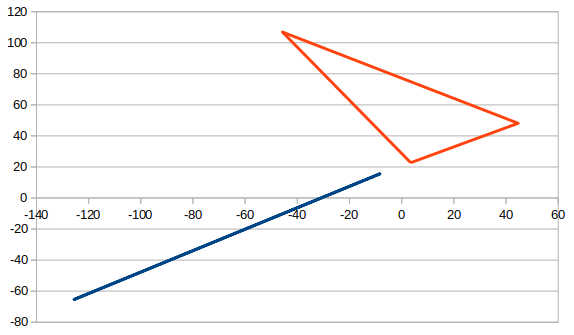
\includegraphics[width=10cm]{./degeneratedFrame.png}\\
\end{figure}
\end{center}

This case can be detected and avoided prior to the intersection test by checking the determinant of the frame: degenerated frames have a null determinant. In the example above the determinant of the first frame is equal to -0.001667.

\subsubsection{2D static}

\begin{scriptsize}
\begin{ttfamily}
\lstinputlisting[breaklines]{../Results/validation2D.txt}
\end{ttfamily}
\end{scriptsize}

\subsubsection{2D dynamic}

\begin{scriptsize}
\begin{ttfamily}
\lstinputlisting[breaklines]{../Results/validation2DTime.txt}
\end{ttfamily}
\end{scriptsize}

\subsubsection{3D static}

\begin{scriptsize}
\begin{ttfamily}
\lstinputlisting[breaklines]{../Results/validation3D.txt}
\end{ttfamily}
\end{scriptsize}

\subsubsection{3D dynamic}

\begin{scriptsize}
\begin{ttfamily}
\lstinputlisting[breaklines]{../Results/validation3DTime.txt}
\end{ttfamily}
\end{scriptsize}

\section{Qualification against SAT}

In this section I introduce the code I've used to qualify the algorithm and its implementation. The qualification consists of running the FMB algorithm on randomly generated pairs of Frame, and check its execution time against the one of running the SAT algorithm on the same pair of Frames.\\

\subsection{Code}

\subsubsection{2D static}

\begin{scriptsize}
\begin{ttfamily}
\lstinputlisting[breaklines]{../2D/qualification.c}
\end{ttfamily}
\end{scriptsize}

\subsubsection{3D static}

\begin{scriptsize}
\begin{ttfamily}
\lstinputlisting[breaklines]{../3D/qualification.c}
\end{ttfamily}
\end{scriptsize}

\subsubsection{2D dynamic}

\begin{scriptsize}
\begin{ttfamily}
\lstinputlisting[breaklines]{../2DTime/qualification.c}
\end{ttfamily}
\end{scriptsize}

\subsubsection{3D dynamic}

\begin{scriptsize}
\begin{ttfamily}
\lstinputlisting[breaklines]{../3DTime/qualification.c}
\end{ttfamily}
\end{scriptsize}

\subsection{Results}

\subsubsection{2D static}

\begin{scriptsize}
\begin{ttfamily}
\lstinputlisting[breaklines]{../Results/qualification2D.txt}
\end{ttfamily}
\end{scriptsize}

\begin{center}
\begin{figure}[H]
\centering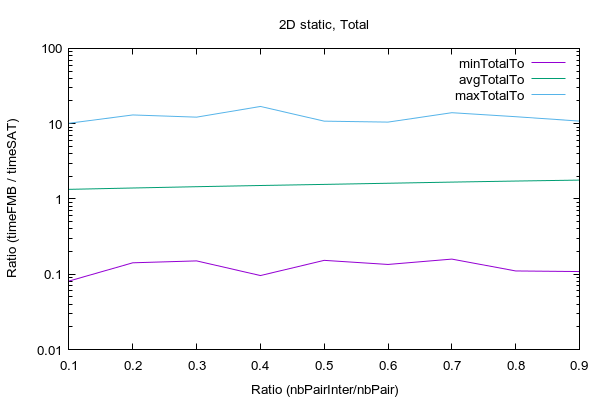
\includegraphics[width=12cm]{../Results/qualification2D.png}\\
\end{figure}
\end{center}

\begin{center}
\begin{figure}[H]
\centering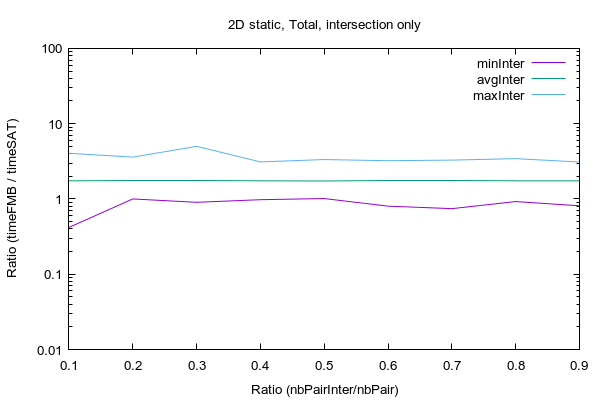
\includegraphics[width=12cm]{../Results/qualification2Dinter.png}\\
\centering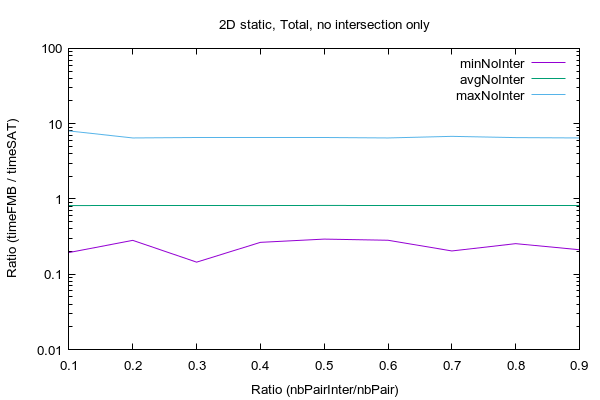
\includegraphics[width=12cm]{../Results/qualification2Dnointer.png}\\
\end{figure}
\end{center}

\begin{center}
\begin{figure}[H]
\centering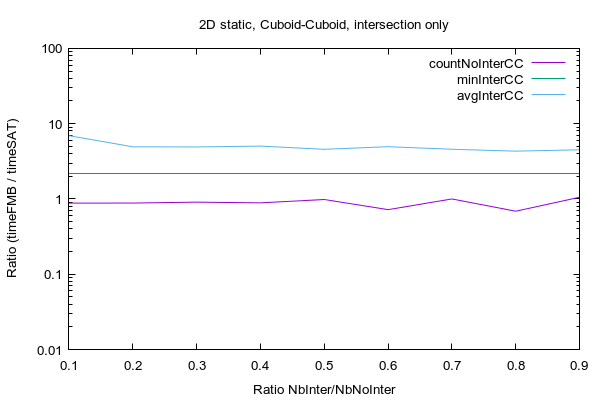
\includegraphics[width=6cm]{../Results/qualification2DCCinter.png}
\centering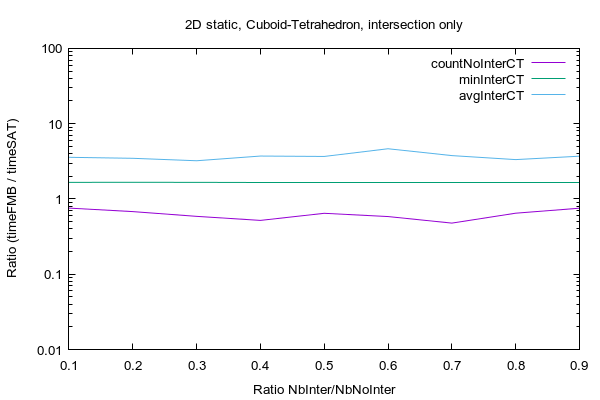
\includegraphics[width=6cm]{../Results/qualification2DCTinter.png}\\
\centering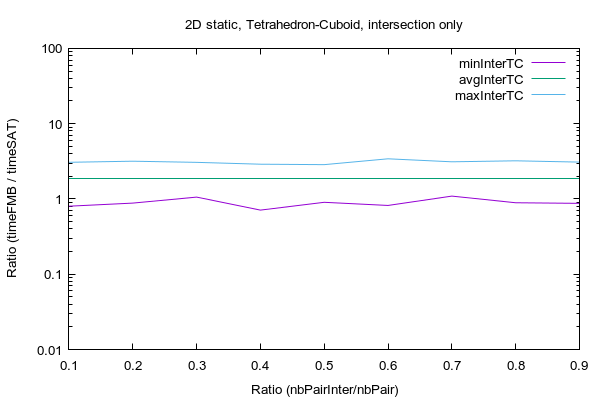
\includegraphics[width=6cm]{../Results/qualification2DTCinter.png}
\centering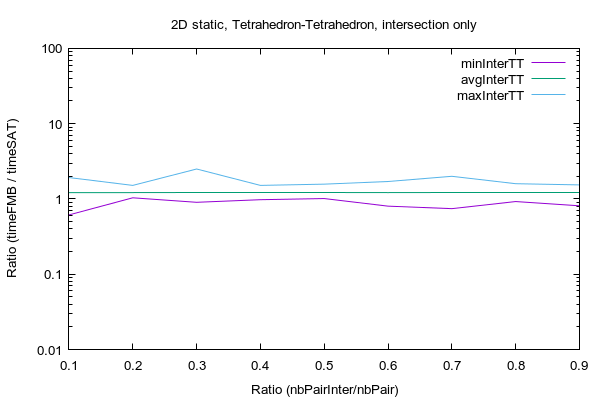
\includegraphics[width=6cm]{../Results/qualification2DTTinter.png}\\
\end{figure}
\end{center}

\begin{center}
\begin{figure}[H]
\centering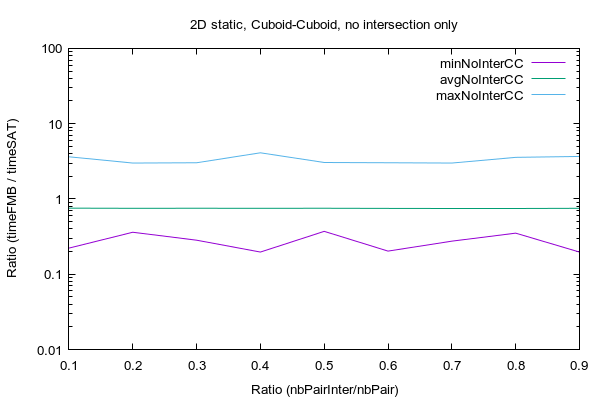
\includegraphics[width=6cm]{../Results/qualification2DCCnointer.png}
\centering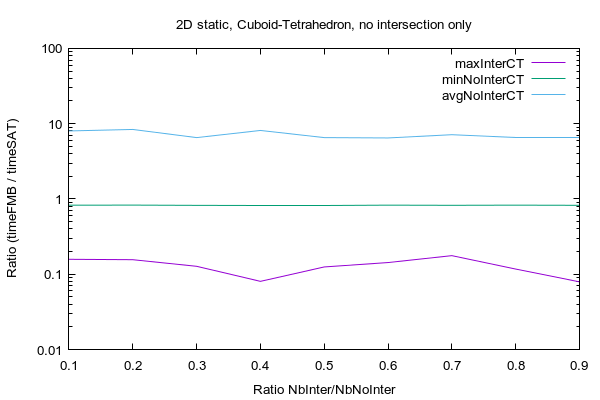
\includegraphics[width=6cm]{../Results/qualification2DCTnointer.png}\\
\centering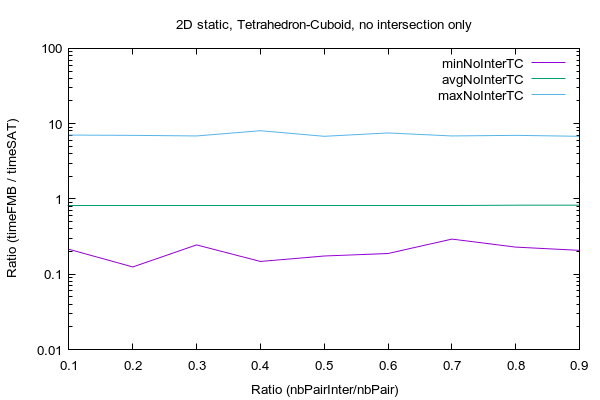
\includegraphics[width=6cm]{../Results/qualification2DTCnointer.png}
\centering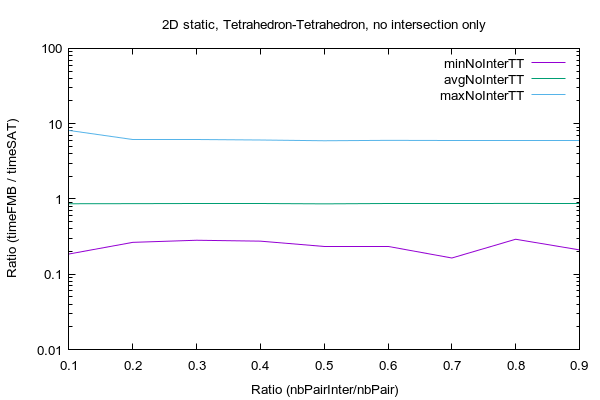
\includegraphics[width=6cm]{../Results/qualification2DTTnointer.png}\\
\end{figure}
\end{center}

\subsubsection{3D static}

\begin{scriptsize}
\begin{ttfamily}
\lstinputlisting[breaklines]{../Results/qualification3D.txt}
\end{ttfamily}
\end{scriptsize}

\begin{center}
\begin{figure}[H]
\centering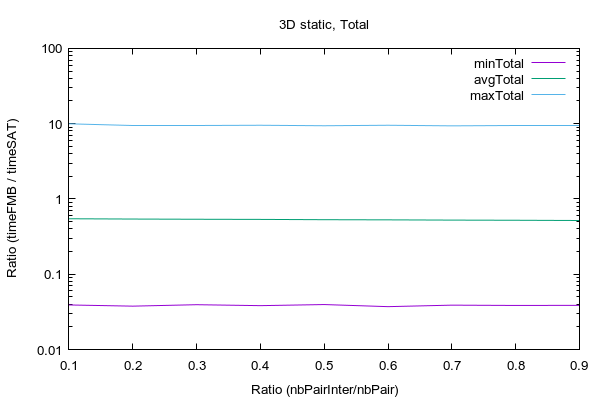
\includegraphics[width=12cm]{../Results/qualification3D.png}\\
\end{figure}
\end{center}

\begin{center}
\begin{figure}[H]
\centering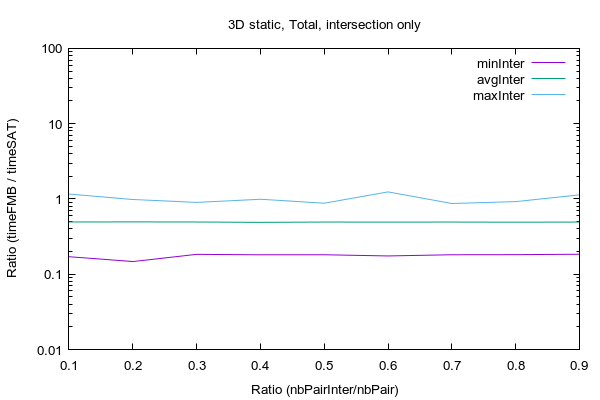
\includegraphics[width=12cm]{../Results/qualification3Dinter.png}\\
\centering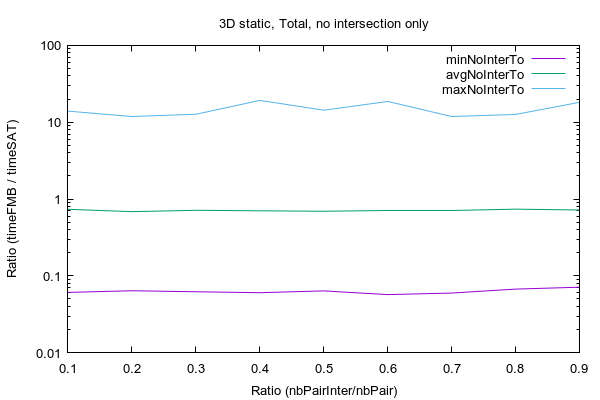
\includegraphics[width=12cm]{../Results/qualification3Dnointer.png}\\
\end{figure}
\end{center}

\begin{center}
\begin{figure}[H]
\centering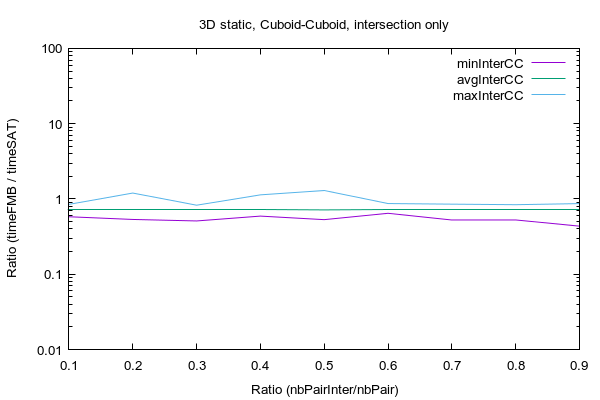
\includegraphics[width=6cm]{../Results/qualification3DCCinter.png}
\centering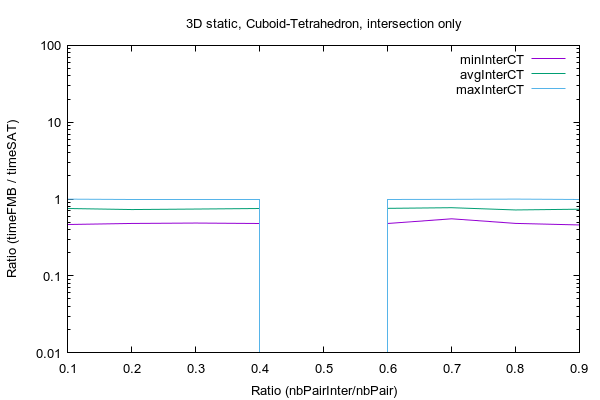
\includegraphics[width=6cm]{../Results/qualification3DCTinter.png}\\
\centering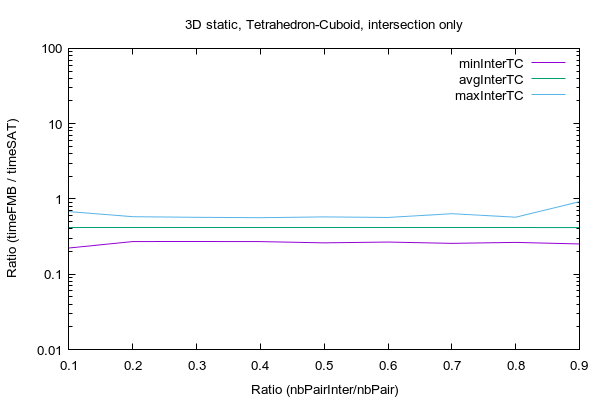
\includegraphics[width=6cm]{../Results/qualification3DTCinter.png}
\centering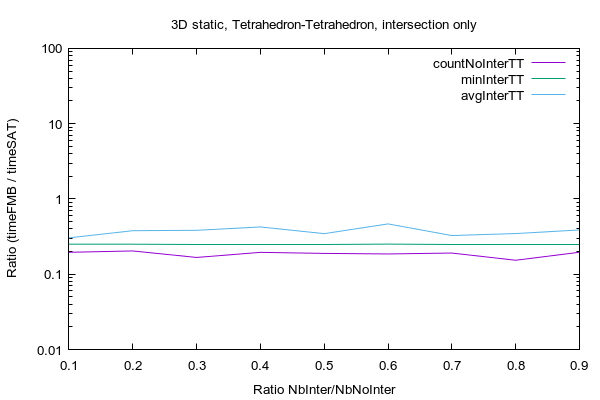
\includegraphics[width=6cm]{../Results/qualification3DTTinter.png}\\
\end{figure}
\end{center}

\begin{center}
\begin{figure}[H]
\centering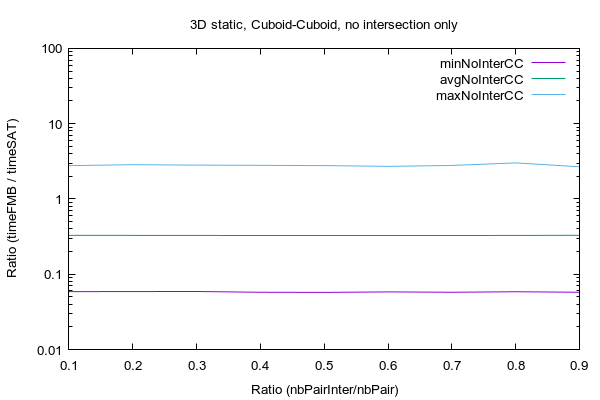
\includegraphics[width=6cm]{../Results/qualification3DCCnointer.png}
\centering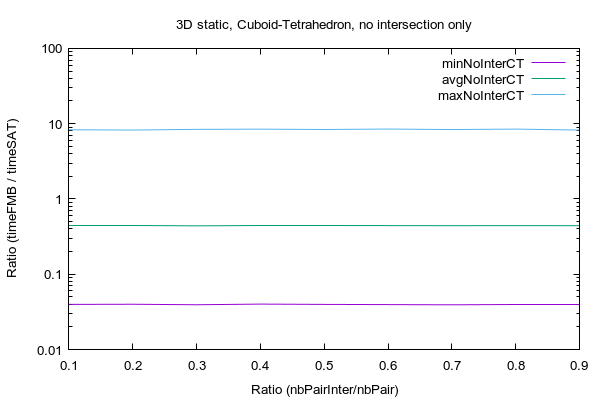
\includegraphics[width=6cm]{../Results/qualification3DCTnointer.png}\\
\centering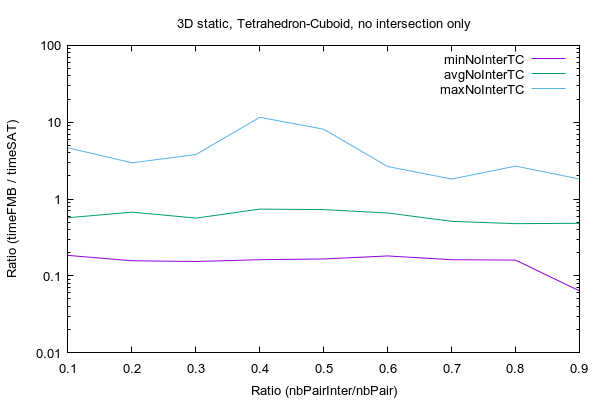
\includegraphics[width=6cm]{../Results/qualification3DTCnointer.png}
\centering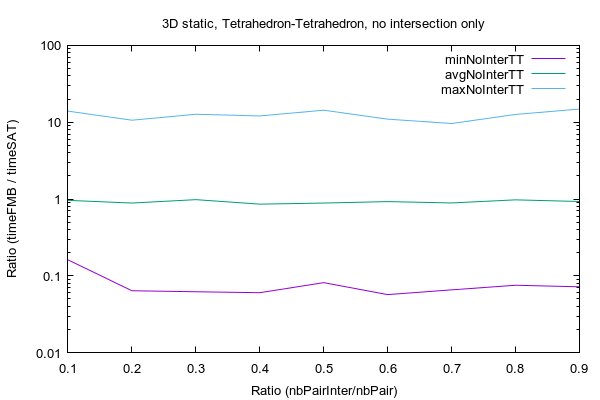
\includegraphics[width=6cm]{../Results/qualification3DTTnointer.png}\\
\end{figure}
\end{center}

\subsubsection{2D dynamic}

\begin{scriptsize}
\begin{ttfamily}
\lstinputlisting[breaklines]{../Results/qualification2DTime.txt}
\end{ttfamily}
\end{scriptsize}

\begin{center}
\begin{figure}[H]
\centering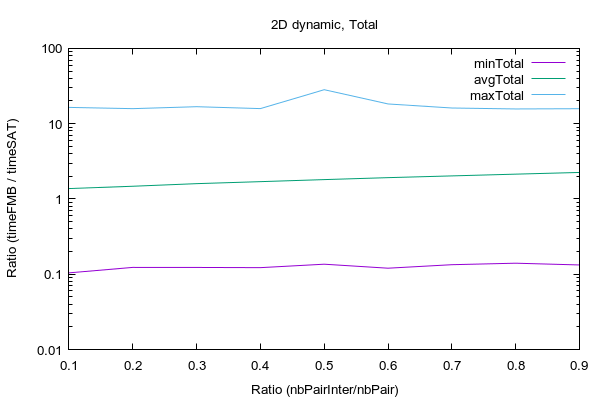
\includegraphics[width=12cm]{../Results/qualification2DTime.png}\\
\end{figure}
\end{center}

\begin{center}
\begin{figure}[H]
\centering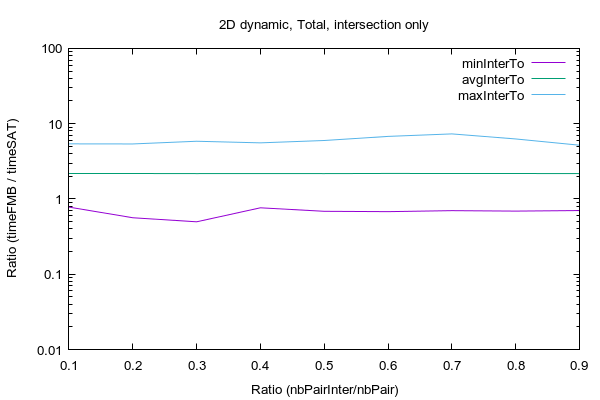
\includegraphics[width=12cm]{../Results/qualification2DTimeinter.png}\\
\centering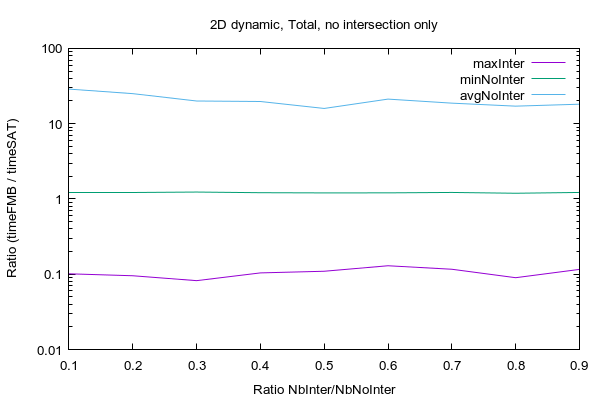
\includegraphics[width=12cm]{../Results/qualification2DTimenointer.png}\\
\end{figure}
\end{center}

\begin{center}
\begin{figure}[H]
\centering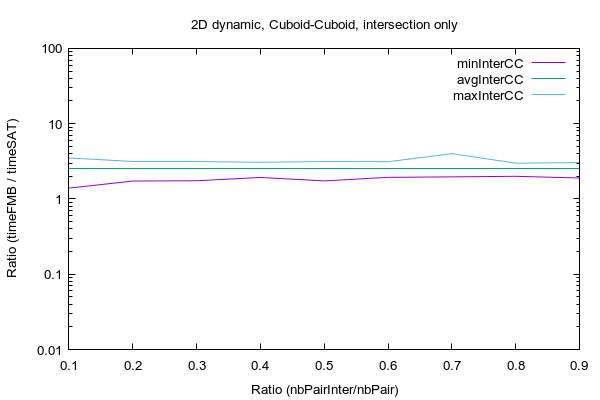
\includegraphics[width=6cm]{../Results/qualification2DTimeCCinter.png}
\centering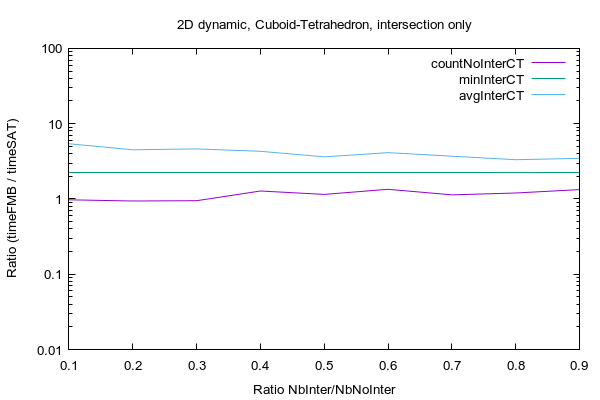
\includegraphics[width=6cm]{../Results/qualification2DTimeCTinter.png}\\
\centering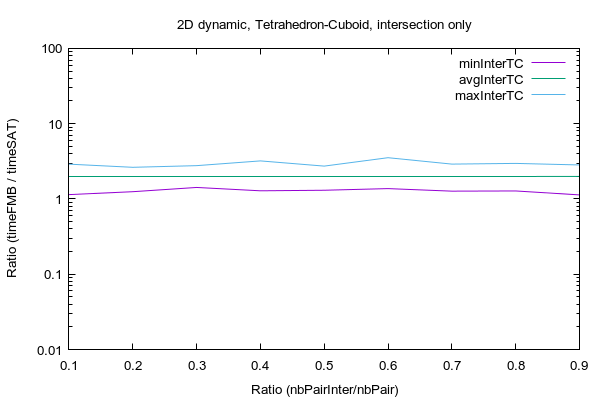
\includegraphics[width=6cm]{../Results/qualification2DTimeTCinter.png}
\centering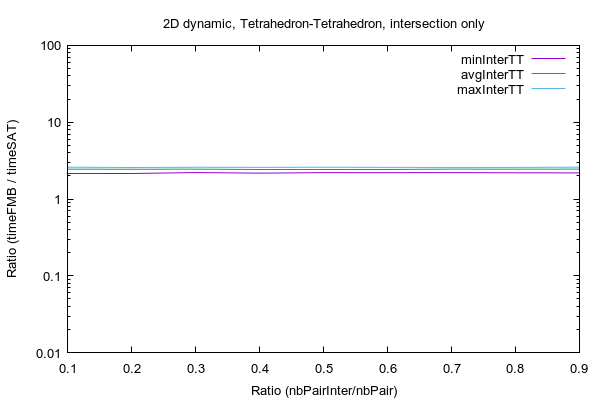
\includegraphics[width=6cm]{../Results/qualification2DTimeTTinter.png}\\
\end{figure}
\end{center}

\begin{center}
\begin{figure}[H]
\centering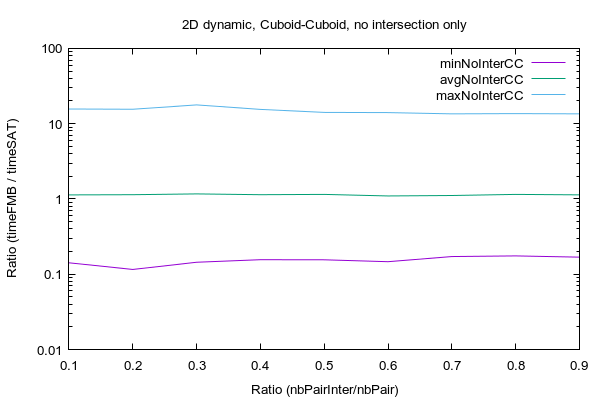
\includegraphics[width=6cm]{../Results/qualification2DTimeCCnointer.png}
\centering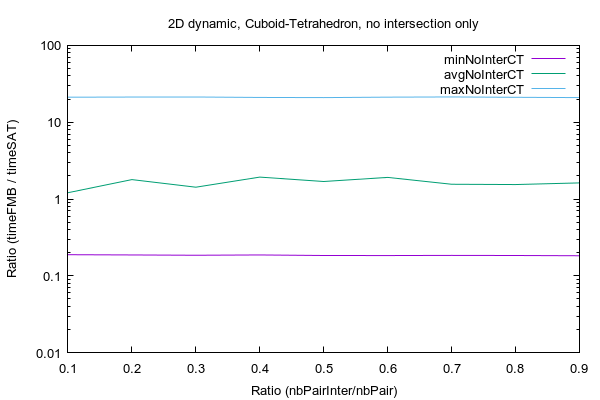
\includegraphics[width=6cm]{../Results/qualification2DTimeCTnointer.png}\\
\centering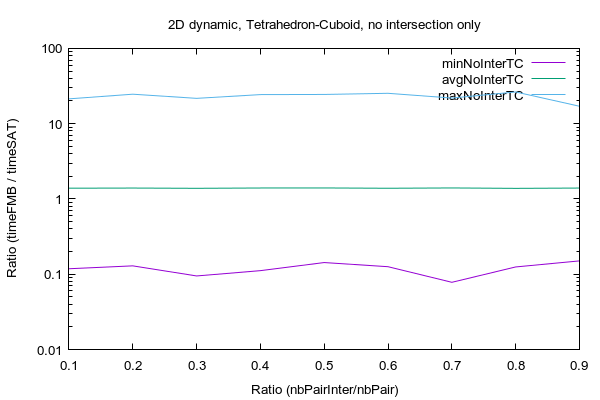
\includegraphics[width=6cm]{../Results/qualification2DTimeTCnointer.png}
\centering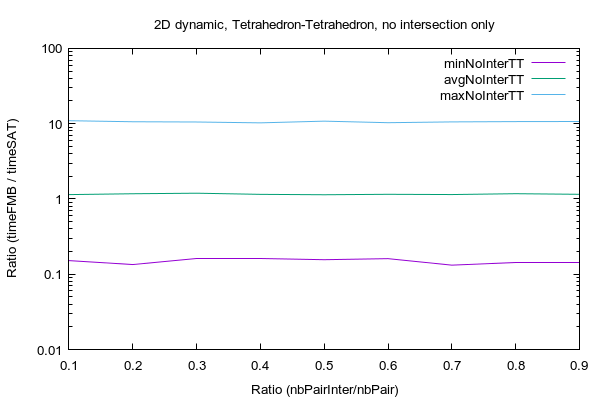
\includegraphics[width=6cm]{../Results/qualification2DTimeTTnointer.png}\\
\end{figure}
\end{center}

\subsubsection{3D dynamic}

\begin{scriptsize}
\begin{ttfamily}
\lstinputlisting[breaklines]{../Results/qualification3DTime.txt}
\end{ttfamily}
\end{scriptsize}

\begin{center}
\begin{figure}[H]
\centering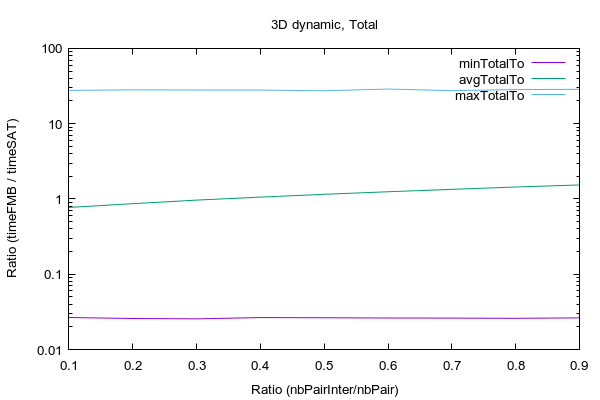
\includegraphics[width=12cm]{../Results/qualification3DTime.png}\\
\end{figure}
\end{center}

\begin{center}
\begin{figure}[H]
\centering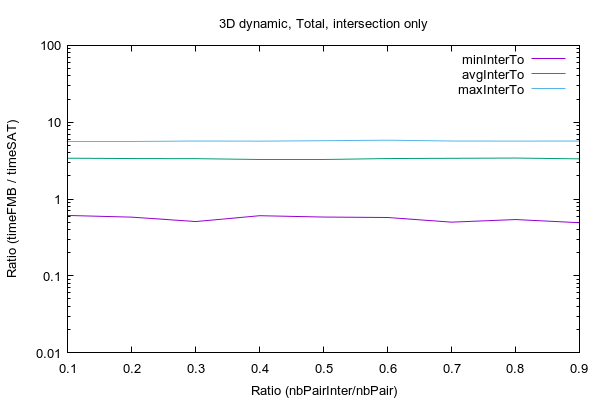
\includegraphics[width=12cm]{../Results/qualification3DTimeinter.png}\\
\centering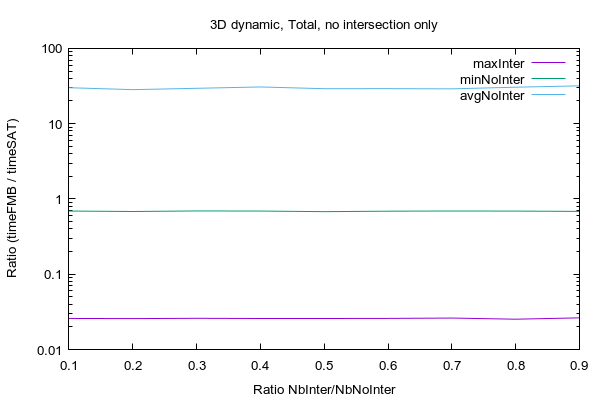
\includegraphics[width=12cm]{../Results/qualification3DTimenointer.png}\\
\end{figure}
\end{center}

\begin{center}
\begin{figure}[H]
\centering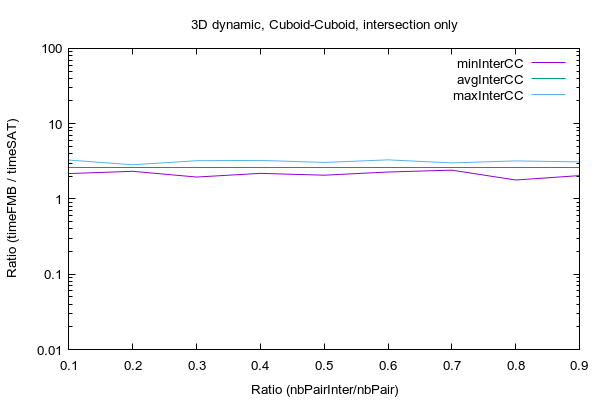
\includegraphics[width=6cm]{../Results/qualification3DTimeCCinter.png}
\centering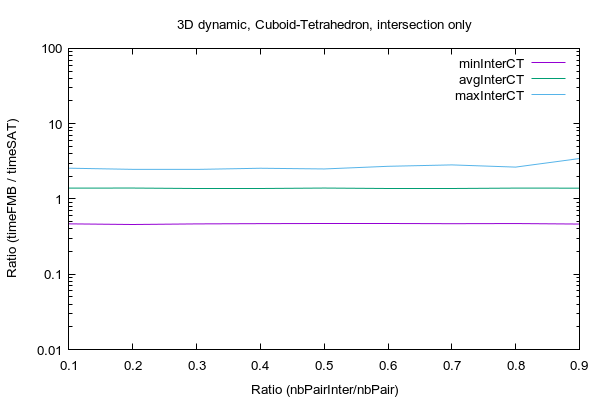
\includegraphics[width=6cm]{../Results/qualification3DTimeCTinter.png}\\
\centering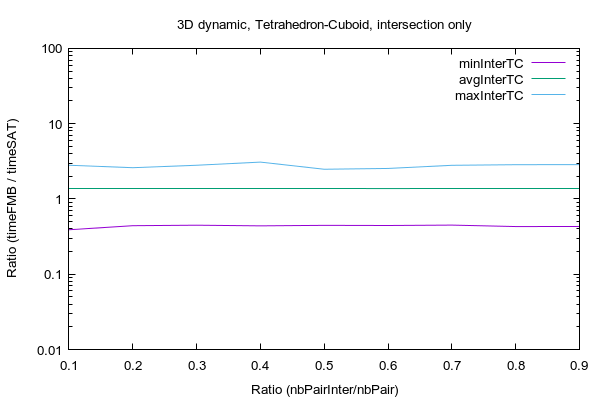
\includegraphics[width=6cm]{../Results/qualification3DTimeTCinter.png}
\centering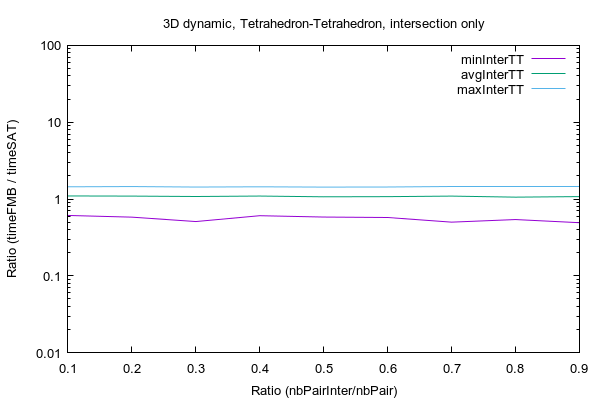
\includegraphics[width=6cm]{../Results/qualification3DTimeTTinter.png}\\
\end{figure}
\end{center}

\begin{center}
\begin{figure}[H]
\centering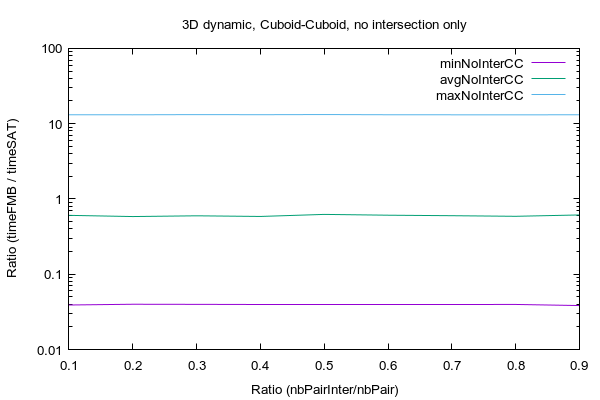
\includegraphics[width=6cm]{../Results/qualification3DTimeCCnointer.png}
\centering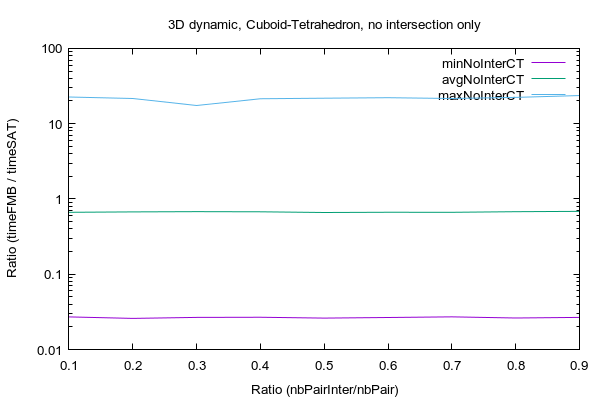
\includegraphics[width=6cm]{../Results/qualification3DTimeCTnointer.png}\\
\centering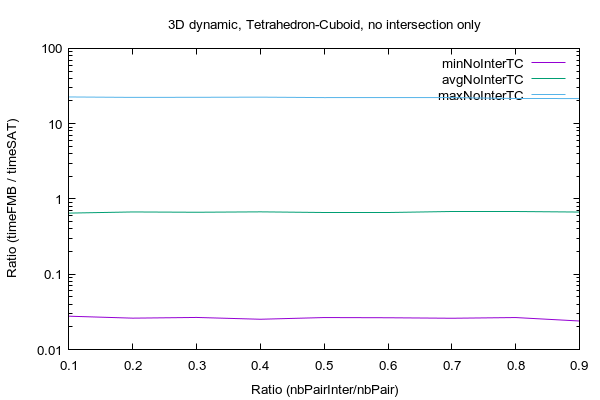
\includegraphics[width=6cm]{../Results/qualification3DTimeTCnointer.png}
\centering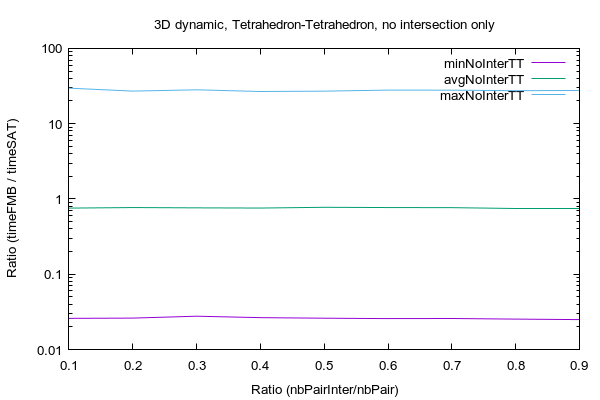
\includegraphics[width=6cm]{../Results/qualification3DTimeTTnointer.png}\\
\end{figure}
\end{center}

\section{Conclusion}

The validation proves that the FMB algorithm correctly identifies intersection of pairs of Frames in accordance with the results of the SAT algorithm.\\

The qualification shows that the FMB is 1.2 to 1.8 times slower than the SAT algorithm in the 2D dynamic case. However it is around 2 times faster in the 3D static case, and up to 1.25 times faster in 3D dynamic and up to 1.1 times faster in the 2D static case if the percentage of tested pairs in intersection is less than, respectively, around 40\% and 25\%.\\

On one given pair of Frame, the relative speed of the FMB algorithm varies widely, from around 20 times slower to 50 times faster. This is explained by the way the 2 algorithms works: they both make the asumption that the Frames are intersecting and run through a series of tests to try to prove it wrong. This leads to best cases and worst cases for both algorithm: a non interesecting detected right from the first test, or one detected by the last test. These best and worst cases are different for the two algorithm as the tests they performed are completely different. But globally, the FMB algorithm has the advantage.\\

\section{Annex}

\subsection{Runtime environment}
\label{runtime_environment}

Results introduce in this paper have been produced by compiling and running the corresponding algorithms in the following environment:\\

\begin{scriptsize}
\begin{ttfamily}
> uname -v
#40~18.04.1-Ubuntu SMP Thu Nov 14 12:06:39 UTC 2019

> lshw -short
H/W path       Device      Class          Description
=====================================================
                           system         VC65-C1
/0                         bus            VC65-C1
/0/0                       memory         64KiB BIOS
/0/2f                      memory         16GiB System Memory
/0/2f/0                    memory         [empty]
/0/2f/1                    memory         16GiB SODIMM DDR4 Synchronous 2400 MHz (0.4 ns)
/0/39                      memory         384KiB L1 cache
/0/3a                      memory         1536KiB L2 cache
/0/3b                      memory         12MiB L3 cache
/0/3c                      processor      Intel(R) Core(TM) i7-8700T CPU @ 2.40GHz
/0/100                     bridge         8th Gen Core Processor Host Bridge/DRAM Registers
/0/100/2                   display        Intel Corporation
/0/100/12                  generic        Cannon Lake PCH Thermal Controller
/0/100/14                  bus            Cannon Lake PCH USB 3.1 xHCI Host Controller
/0/100/14/0    usb1        bus            xHCI Host Controller
/0/100/14/0/5              input          ELECOM Wired Keyboard
/0/100/14/0/6              input          PTZ-630
/0/100/14/0/7              generic        USB2.0-CRW
/0/100/14/0/e              communication  Bluetooth wireless interface
/0/100/14/1    usb2        bus            xHCI Host Controller
/0/100/14.2                memory         RAM memory
/0/100/14.3    wlo1        network        Wireless-AC 9560 [Jefferson Peak]
/0/100/16                  communication  Cannon Lake PCH HECI Controller
/0/100/17                  storage        Cannon Lake PCH SATA AHCI Controller
/0/100/1f                  bridge         Intel Corporation
/0/100/1f.3                multimedia     Cannon Lake PCH cAVS
/0/100/1f.4                bus            Cannon Lake PCH SMBus Controller
/0/100/1f.5                bus            Cannon Lake PCH SPI Controller
/0/100/1f.6    eno2        network        Ethernet Connection (7) I219-V
/0/1           scsi0       storage        
/0/1/0.0.0     /dev/sda    disk           128GB HFS128G39TND-N21
/0/1/0.0.0/1               volume         99MiB Windows FAT volume
/0/1/0.0.0/2   /dev/sda2   volume         15MiB reserved partition
/0/1/0.0.0/3   /dev/sda3   volume         83GiB Windows NTFS volume
/0/1/0.0.0/4   /dev/sda4   volume         499MiB Windows NTFS volume
/0/1/0.0.0/5   /dev/sda5   volume         35GiB EXT4 volume
/0/2           scsi2       storage        
/0/2/0.0.0     /dev/sdb    disk           500GB ST500LM034-2GH17
/0/2/0.0.0/1   /dev/sdb1   volume         463GiB EXT4 volume
/0/2/0.0.0/2   /dev/sdb2   volume         499MiB Windows FAT volume
/0/3           scsi5       storage        
/0/3/0.0.0     /dev/cdrom  disk           BD-RE BU50N
/1                         power          To Be Filled By O.E.M.

> lscpu
Architecture:        x86_64
CPU op-mode(s):      32-bit, 64-bit
Byte Order:          Little Endian
CPU(s):              12
On-line CPU(s) list: 0-11
Thread(s) per core:  2
Core(s) per socket:  6
Socket(s):           1
NUMA node(s):        1
Vendor ID:           GenuineIntel
CPU family:          6
Model:               158
Model name:          Intel(R) Core(TM) i7-8700T CPU @ 2.40GHz
Stepping:            10
CPU MHz:             1380.998
CPU max MHz:         4000.0000
CPU min MHz:         800.0000
BogoMIPS:            4800.00
Virtualization:      VT-x
L1d cache:           32K
L1i cache:           32K
L2 cache:            256K
L3 cache:            12288K
NUMA node0 CPU(s):   0-11
Flags:               fpu vme de pse tsc msr pae mce cx8 apic sep mtrr pge mca cmov pat pse36 clflush dts acpi mmx fxsr sse sse2 ss ht tm pbe syscall nx pdpe1gb rdtscp lm constant_tsc art arch_perfmon pebs bts rep_good nopl xtopology nonstop_tsc cpuid aperfmperf tsc_known_freq pni pclmulqdq dtes64 monitor ds_cpl vmx smx est tm2 ssse3 sdbg fma cx16 xtpr pdcm pcid sse4_1 sse4_2 x2apic movbe popcnt tsc_deadline_timer aes xsave avx f16c rdrand lahf_lm abm 3dnowprefetch cpuid_fault epb invpcid_single pti ssbd ibrs ibpb stibp tpr_shadow vnmi flexpriority ept vpid ept_ad fsgsbase tsc_adjust bmi1 hle avx2 smep bmi2 erms invpcid rtm mpx rdseed adx smap clflushopt intel_pt xsaveopt xsavec xgetbv1 xsaves dtherm ida arat pln pts hwp hwp_notify hwp_act_window hwp_epp md_clear flush_l1d

> gcc -v
Using built-in specs.
COLLECT_GCC=gcc
COLLECT_LTO_WRAPPER=/usr/lib/gcc/x86_64-linux-gnu/7/lto-wrapper
OFFLOAD_TARGET_NAMES=nvptx-none
OFFLOAD_TARGET_DEFAULT=1
Target: x86_64-linux-gnu
Configured with: ../src/configure -v --with-pkgversion='Ubuntu 7.4.0-1ubuntu1~18.04.1' --with-bugurl=file:///usr/share/doc/gcc-7/README.Bugs --enable-languages=c,ada,c++,go,brig,d,fortran,objc,obj-c++ --prefix=/usr --with-gcc-major-version-only --program-suffix=-7 --program-prefix=x86_64-linux-gnu- --enable-shared --enable-linker-build-id --libexecdir=/usr/lib --without-included-gettext --enable-threads=posix --libdir=/usr/lib --enable-nls --with-sysroot=/ --enable-clocale=gnu --enable-libstdcxx-debug --enable-libstdcxx-time=yes --with-default-libstdcxx-abi=new --enable-gnu-unique-object --disable-vtable-verify --enable-libmpx --enable-plugin --enable-default-pie --with-system-zlib --with-target-system-zlib --enable-objc-gc=auto --enable-multiarch --disable-werror --with-arch-32=i686 --with-abi=m64 --with-multilib-list=m32,m64,mx32 --enable-multilib --with-tune=generic --enable-offload-targets=nvptx-none --without-cuda-driver --enable-checking=release --build=x86_64-linux-gnu --host=x86_64-linux-gnu --target=x86_64-linux-gnu
Thread model: posix
gcc version 7.4.0 (Ubuntu 7.4.0-1ubuntu1~18.04.1) 
\end{ttfamily}
\end{scriptsize}


\subsection{SAT implementation}
\label{sat_implementation}

In this section I introduce the code of the implementation of the SAT algorithm, used to validate and qualify the FMB algorithm.\\

\subsubsection{Header}

\begin{scriptsize}
\begin{ttfamily}
\lstinputlisting[breaklines]{../SAT/sat.h}
\end{ttfamily}
\end{scriptsize}

\subsubsection{Body}

\begin{scriptsize}
\begin{ttfamily}
\lstinputlisting[breaklines]{../SAT/sat.c}
\end{ttfamily}
\end{scriptsize}

\subsection{Makefile}

In this section I introduce the Makefile used to compile the code given in the previous sections.\\

\begin{scriptsize}
\begin{ttfamily}
\lstinputlisting[breaklines]{../Makefile}
\end{ttfamily}
\end{scriptsize}

\subsubsection{2D static}

\begin{scriptsize}
\begin{ttfamily}
\lstinputlisting[breaklines]{../2D/Makefile}
\end{ttfamily}
\end{scriptsize}

\subsubsection{3D static}

\begin{scriptsize}
\begin{ttfamily}
\lstinputlisting[breaklines]{../3D/Makefile}
\end{ttfamily}
\end{scriptsize}

\subsubsection{2D dynamic}

\begin{scriptsize}
\begin{ttfamily}
\lstinputlisting[breaklines]{../2DTime/Makefile}
\end{ttfamily}
\end{scriptsize}

\subsubsection{3D dynamic}

\begin{scriptsize}
\begin{ttfamily}
\lstinputlisting[breaklines]{../3DTime/Makefile}
\end{ttfamily}
\end{scriptsize}

\begin{thebibliography}{9}
\bibitem{fourier} J.J.-B. Fourier. Oeuvres II. Paris, 1890
\bibitem{motzkin} T.S. Motzkin. {\em Beitr\"{a}ge zur Theorie der linearen Ungleichungen}. Thesis, 1936. Reprinted in: {\em Theodore S. Motzkin: selected papers} (D.Cantor et al., eds,), Birkh\"{a}user, Boston, 1983.
\end{thebibliography}

\end{document}
